\documentclass{beamer}
\setbeamertemplate{navigation symbols}{}
\usepackage[latin1]{inputenc}
\usepackage{setspace,dsfont}
\usepackage{amsmath,amssymb,pdfpages}
\usepackage[longnamesfirst,nonamebreak]{natbib}
\usepackage[english]{babel}
\usepackage{eurosym,multirow,hyperref,cmll}
\usepackage{listings}
\usepackage{verbatim,booktabs}

\newcommand{\Lik}{\mathcal{L}}
\newcommand{\lau}{\lambda_u}
\newcommand{\wi}{\underline{w}}
\newcommand{\m}{\mathcal{M}}
\newcommand{\wa}{\overline{w}}
\newcommand{\lae}{\lambda_e}
\newcommand{\1}{\mathbb{1}}
\newcommand{\F}{\mathcal{F}}
\newcommand{\D}{\mathcal{D}}
\newcommand{\f}{\mathfrak{f}}
\newcommand{\E}{\mathbb{E}}
\newcommand{\V}{\mathbb{V}}
\newcommand{\N}{\mathbb{N}}
\newcommand{\Real}{\mathbb{R}}
\newcommand{\X}{\mathcal{X}}
\newcommand{\A}{\mathcal{A}}
\newcommand{\B}{\mathcal{B}}
\newcommand{\hy}{\hat{y}}

\hypersetup{
    colorlinks,%
    citecolor=blue,%
    filecolor=blue,%
    linkcolor=blue,%
    urlcolor=blue,
}
%\usetheme{Boadilla}
%\usetheme{Marburg}
%\usetheme{Hannover}
%\usetheme{Pittsburgh}
%\usetheme{umbc1}
%\usetheme{Montpellier}
%\usetheme{Singapore}
%\usetheme{}
%\usetheme{}
%\lstset {language=C++}

\DeclareMathOperator{\plim}{plim}
\DeclareMathAlphabet{\mathpzc}{OT1}{pzc}{m}{it}

\beamersetuncovermixins{\opaqueness<1>{25}}{\opaqueness<2->{15}}
\begin{document}
\begin{frame}
\title{ECON 613: Applied Econometrics}
\subtitle{Methods for Panel Data}
\titlepage
\end{frame}

\section{Linear Models}

\begin{frame}
\tableofcontents[currentsection] 
\end{frame}

\begin{frame}\frametitle{Introduction (1)}
\begin{itemize}
 \item Data on cross section that is observed over several unit of time.  
 \item In microeconometrics, panel are usually short. 
\end{itemize}
\end{frame}

\begin{frame}\frametitle{Introduction (2)}
\begin{itemize}
\item The error is correlated over time..
\item Examples
\item Open possibilities..
\end{itemize}
\end{frame}

\begin{frame}\frametitle{Introduction (3)}
Consider the following Model
\begin{equation}
 Y_{it} = \alpha_i + \gamma_{j(t)} + \beta X_{it} + \epsilon_{it}
\end{equation}
\begin{itemize}
 \item Estimation of fixed effects
 \item Correlation between the fixed effects
 \item Estimation issues
\end{itemize}
\end{frame}

\begin{frame}\frametitle{Introduction (4)}
Consider the following DGP:
\begin{itemize}
 \item 1,000 individuals over 10 periods. 
 \item $Y_{it} = \alpha_i + \beta X_{it} + \epsilon_{it}$
 \item Parametrization 
 \begin{itemize}
  \item $\beta = 1$
  \item $\alpha_i \sim uniform(0,1)$
  \item $\epsilon_i\sim \N(0,1)$
 \end{itemize}
\end{itemize}
\end{frame}

\begin{frame}\frametitle{Pooled Estimation}
\begin{table}
\begin{center}
\begin{tabular}{l c }
\hline
 & Model 1 \\
\hline
(Intercept) & $0.49^{***}$ \\
            & $(0.02)$     \\
c(xMat)     & $0.93^{***}$ \\
            & $(0.00)$     \\
\hline
R$^2$       & 0.87         \\
Adj. R$^2$  & 0.87         \\
Num. obs.   & 10000        \\
RMSE        & 1.05         \\
\hline
\multicolumn{2}{l}{\scriptsize{$^{***}p<0.001$, $^{**}p<0.01$, $^*p<0.05$}}
\end{tabular}
\caption{Statistical models}
\label{table:coefficients}
\end{center}
\end{table}
\end{frame}

\begin{frame}\frametitle{Fitted Values (1)}
\begin{figure}
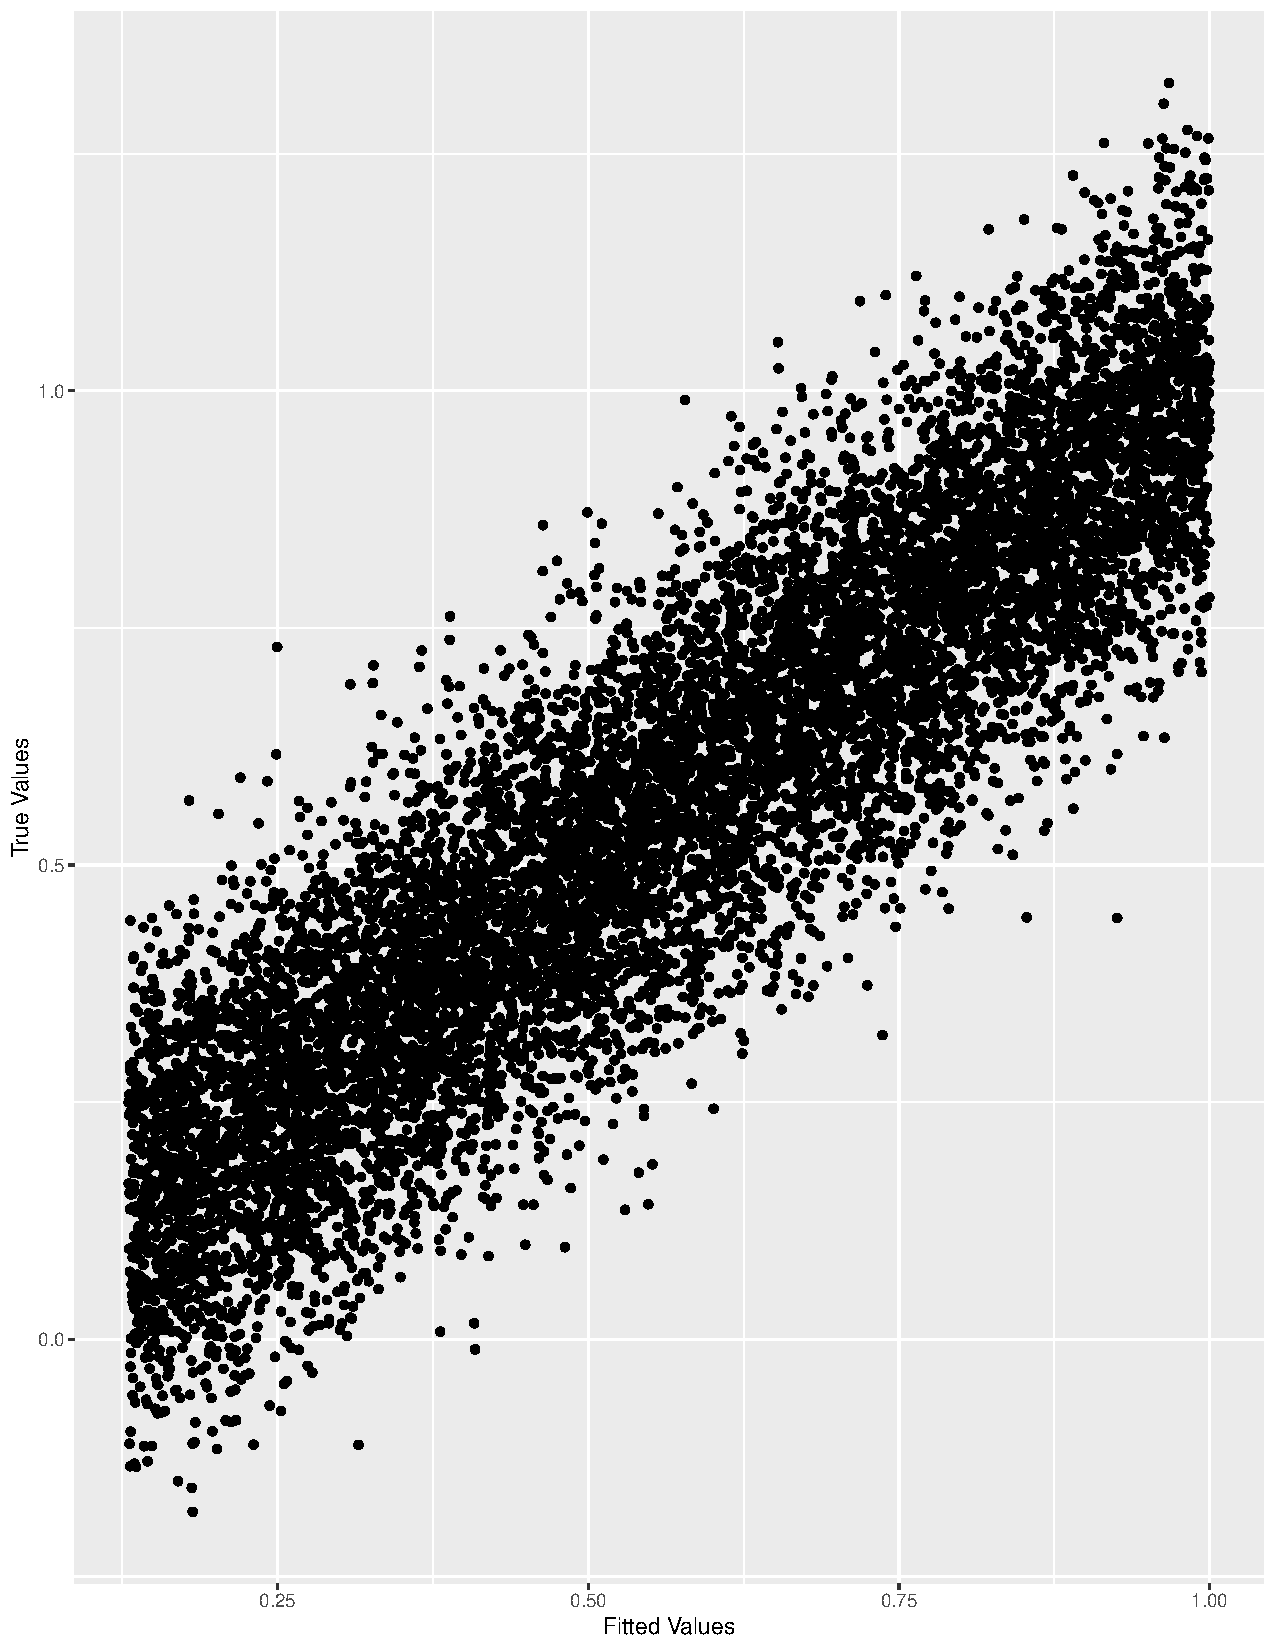
\includegraphics[width = 5cm]{plot/reg1}
\end{figure}
\end{frame}


\begin{frame}\frametitle{Introduction (5)}
Consider the following DGP:
\begin{itemize}
 \item 1,000 individuals over 10 periods. 
 \item $Y_{it} = \alpha_i + \beta X_{it} + \epsilon_{it}$
 \item Parametrization 
 \begin{itemize}
  \item $\beta = 1$
  \item $\alpha_i \sim uniform(-10,10)$
  \item $\epsilon_i \sim \N(0,1)$
 \end{itemize}
\end{itemize}
\end{frame}

\begin{frame}\frametitle{Pooled Estimation}
\begin{table}
\begin{center}
\begin{tabular}{l c }
\hline
 & Model 1 \\
\hline
(Intercept) & $-0.26^{*}$  \\
            & $(0.11)$     \\
c(xMat)     & $0.40^{***}$ \\
            & $(0.02)$     \\
\hline
R$^2$       & 0.04         \\
Adj. R$^2$  & 0.04         \\
Num. obs.   & 10000        \\
RMSE        & 5.73         \\
\hline
\multicolumn{2}{l}{\scriptsize{$^{***}p<0.001$, $^{**}p<0.01$, $^*p<0.05$}}
\end{tabular}
\caption{Statistical models}
\label{table:coefficients}
\end{center}
\end{table}
\end{frame}


\begin{frame}\frametitle{Fitted Values (2)}
\begin{figure}
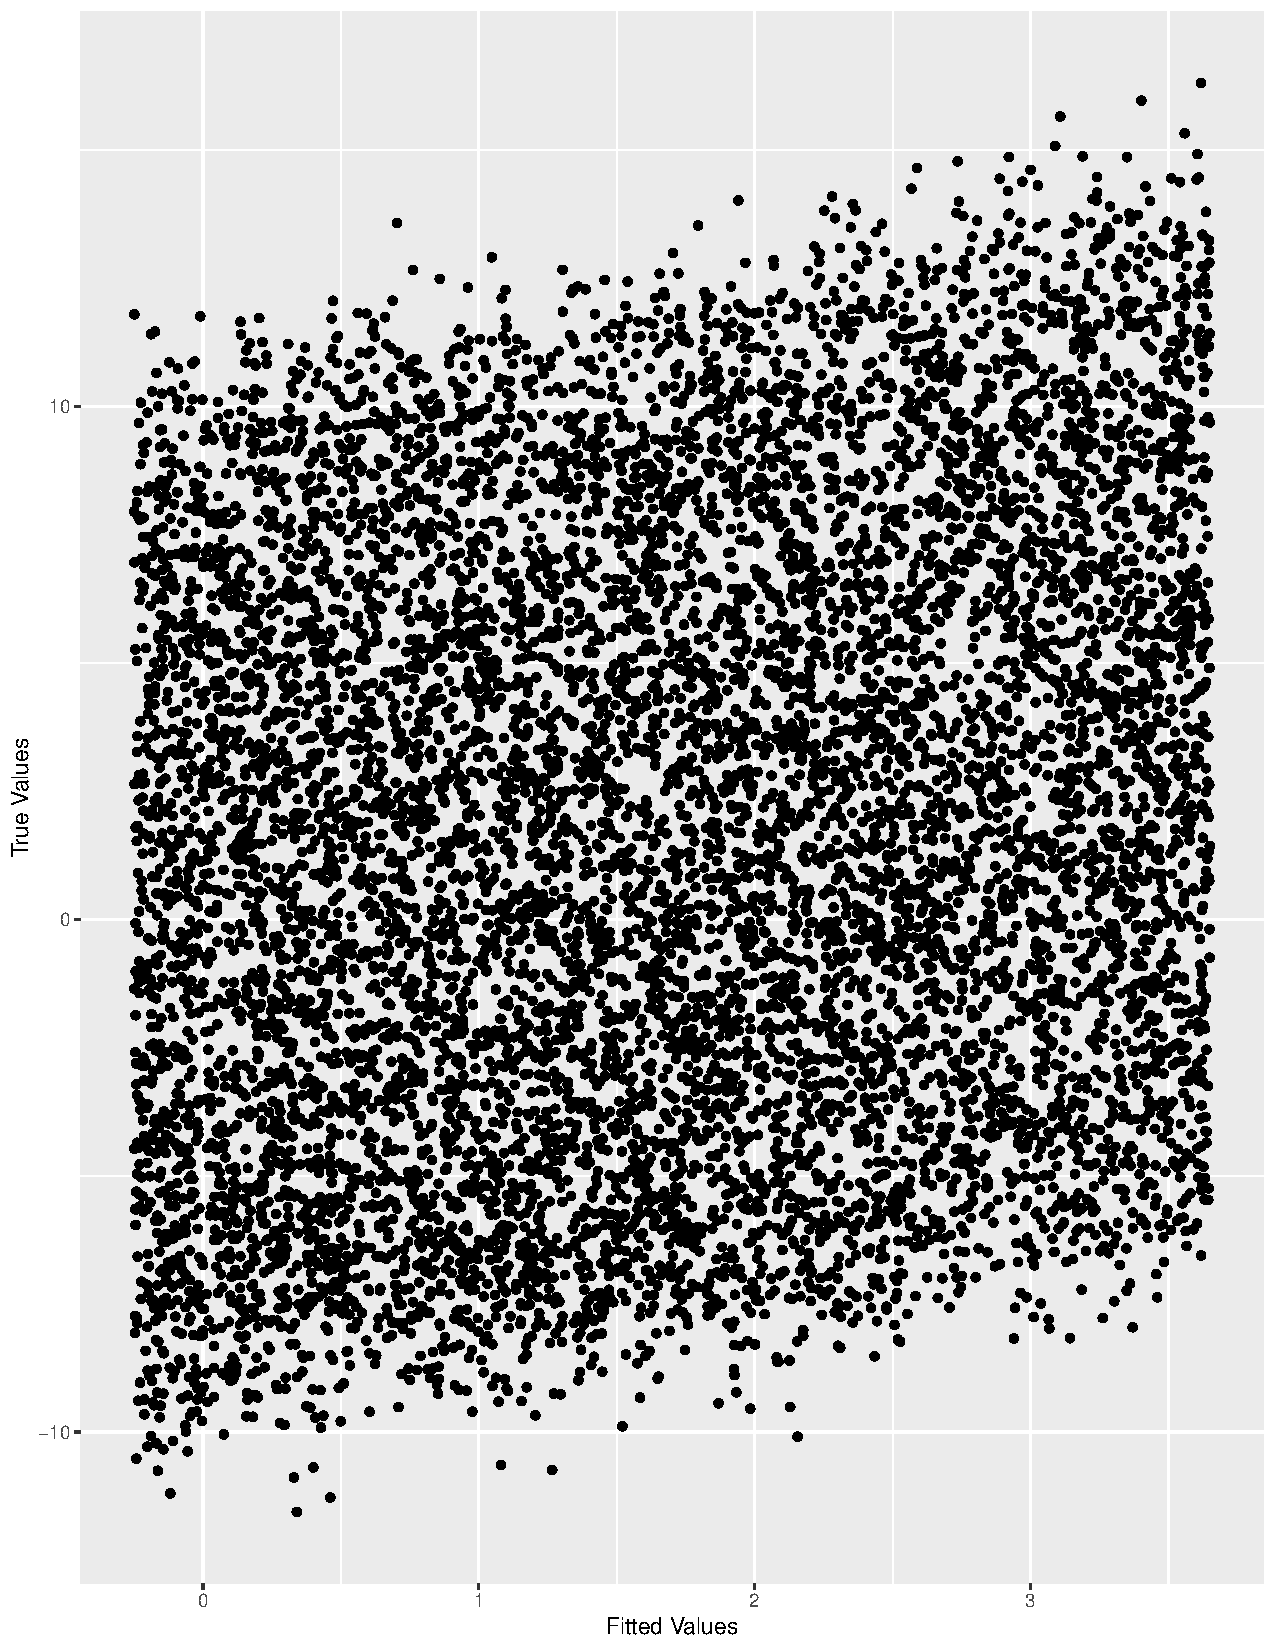
\includegraphics[width = 5cm]{plot/reg2}
\end{figure}
\end{frame}

\begin{frame}\frametitle{Effects}
\begin{itemize}
 \item Pooled Estimation is a good starting point.
 \item Individual VS Time Effect.
\end{itemize}
\end{frame}

\begin{frame}\frametitle{Individual Effects}
\begin{itemize}
 \item Fixed Effects
 \item Random Effects
 \item Examples: Return to Education
\end{itemize}
\end{frame}

\begin{frame}\frametitle{Time Effects}
\begin{itemize}
 \item Long Panel Case
 \item Example: Seasonality? 
\end{itemize}
\end{frame}

\begin{frame}\frametitle{Some Models (1)}
\begin{itemize}
 \item Pooled Estimator
 \begin{equation}
  Y_{it} = \alpha + \beta X_{it} + \epsilon_{it}
 \end{equation}
\item Problems
\end{itemize}
\end{frame}

\begin{frame}\frametitle{Some Models (2)}
\begin{itemize}
 \item Between Estimator
 \begin{equation}
  \bar{y}_i = \alpha_i + \beta \bar{x}_{i} + \bar{\epsilon}_{i}
 \end{equation}
\item Problems
\end{itemize}
\end{frame}

\begin{frame}\frametitle{Some Models (3)}
\begin{itemize}
 \item Within Estimator
 \begin{equation}
 y_{it} - \bar{y}_i =  \beta (x_{it} - \bar{x}_{i}) + 
 (\epsilon_{it} - \bar{\epsilon}_{i})
 \end{equation}
\item Problems
\end{itemize}
\end{frame}

\begin{frame}\frametitle{Some Models (4)}
\begin{itemize}
 \item First Difference Estimator
 \begin{equation}
 y_{it} - y_{i,t-1} =  \beta (x_{it} - x_{i,t-1}) + 
 (\epsilon_{it} - \epsilon_{i,t-1})
 \end{equation}
\item Problems
\end{itemize}

\end{frame}

\subsection{Applications}

\begin{frame}\frametitle{More Guns, Less Crime}
\begin{quote}
In a remarkable paper published in 1997, John Lott and David Mustard managed
to set the agenda for much subsequent work on the impact of guns on crime in America
by creating a massive data set of crime across all U.S. counties from 1977 through 1992
and amassing a powerful statistical argument that state laws enabling citizens to carry
concealed handguns had reduced crime.1
 The initial paper was followed a year later by
an even more comprehensive and sustained argument to the same effect in a book solely
authored by John Lott entitled More Guns, Less Crime (now in its second edition). 
\end{quote}
\end{frame}


\begin{frame}\frametitle{Data: Guns}
A data frame containing 1,173 observations on 13 variables.
\begin{itemize}
 \item state: factor indicating state.
\item year: factor indicating year.
\item violent: violent crime rate (incidents per 100,000 members of the population).
\item murder: murder rate (incidents per 100,000).
\item robbery: robbery rate (incidents per 100,000).
\item prisoners: incarceration rate in the state in the previous year 
\item afam: percent of state population that is African-American
\item cauc: percent of state population that is Caucasian, \item male: percent of state population that is male
\item population: state population, in millions of people.
\item income: real per capita personal income in the state (US \$).
\item density population per square mile of land area, divided by 1,000.
\item law factor. Does the state have a shall carry law in effect in that year?
\end{itemize}
\end{frame}

\begin{frame}\frametitle{Overtime Variation}
\begin{figure}
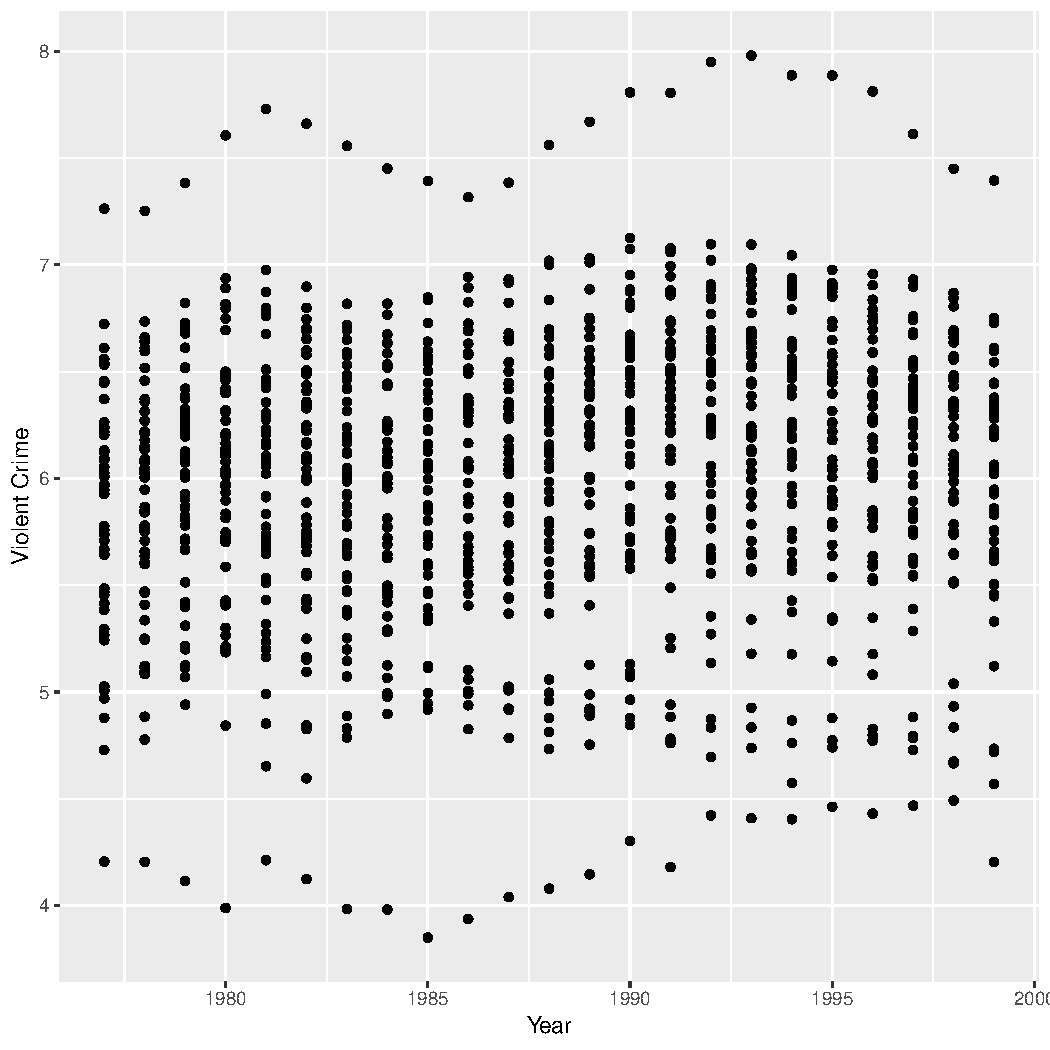
\includegraphics[width = 9cm]{plot/Time}
\end{figure}
\end{frame}


\begin{frame}\frametitle{Cross-sectional Variation (1)}
\begin{figure}
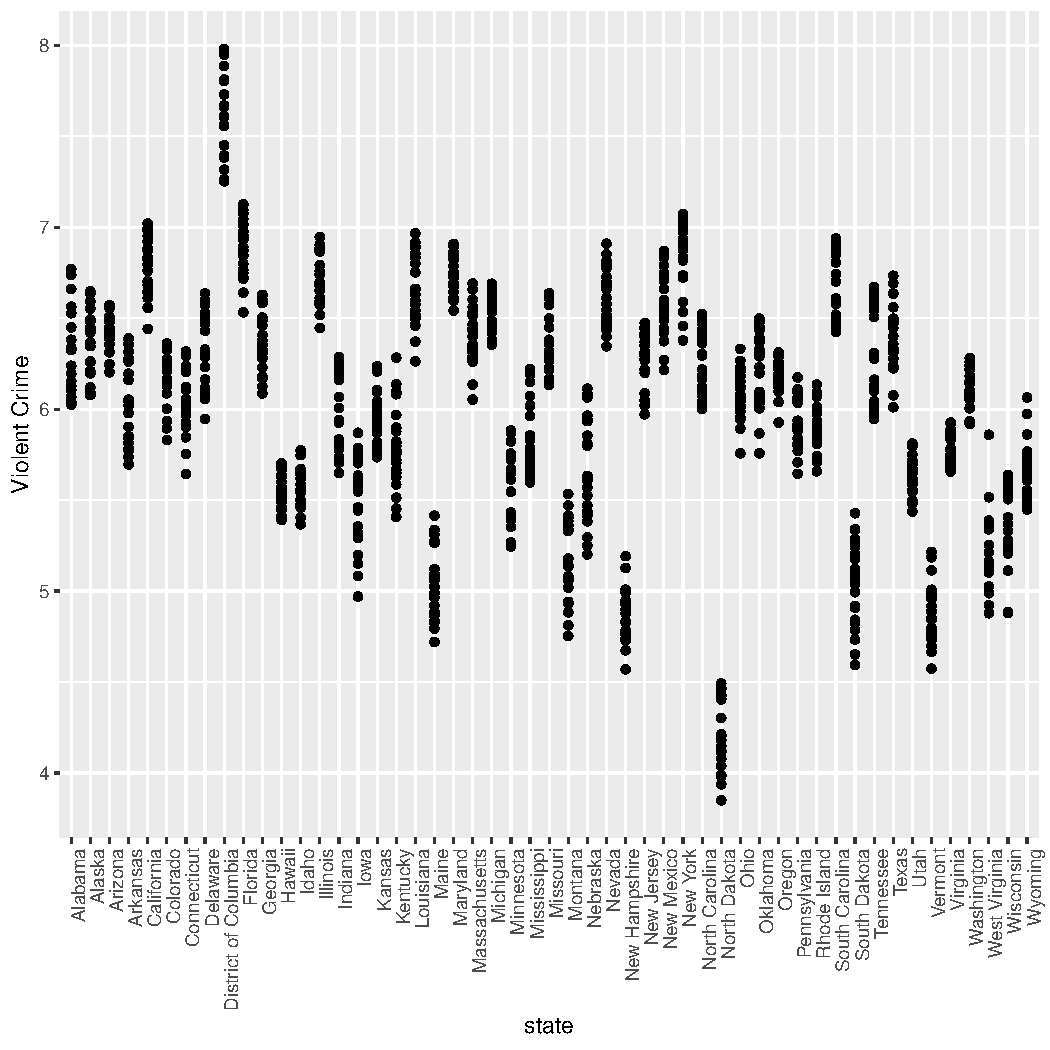
\includegraphics[width = 8cm]{plot/State}
\end{figure}
\end{frame}

\begin{frame}\frametitle{Cross-sectional Variation (2)}
\begin{figure}
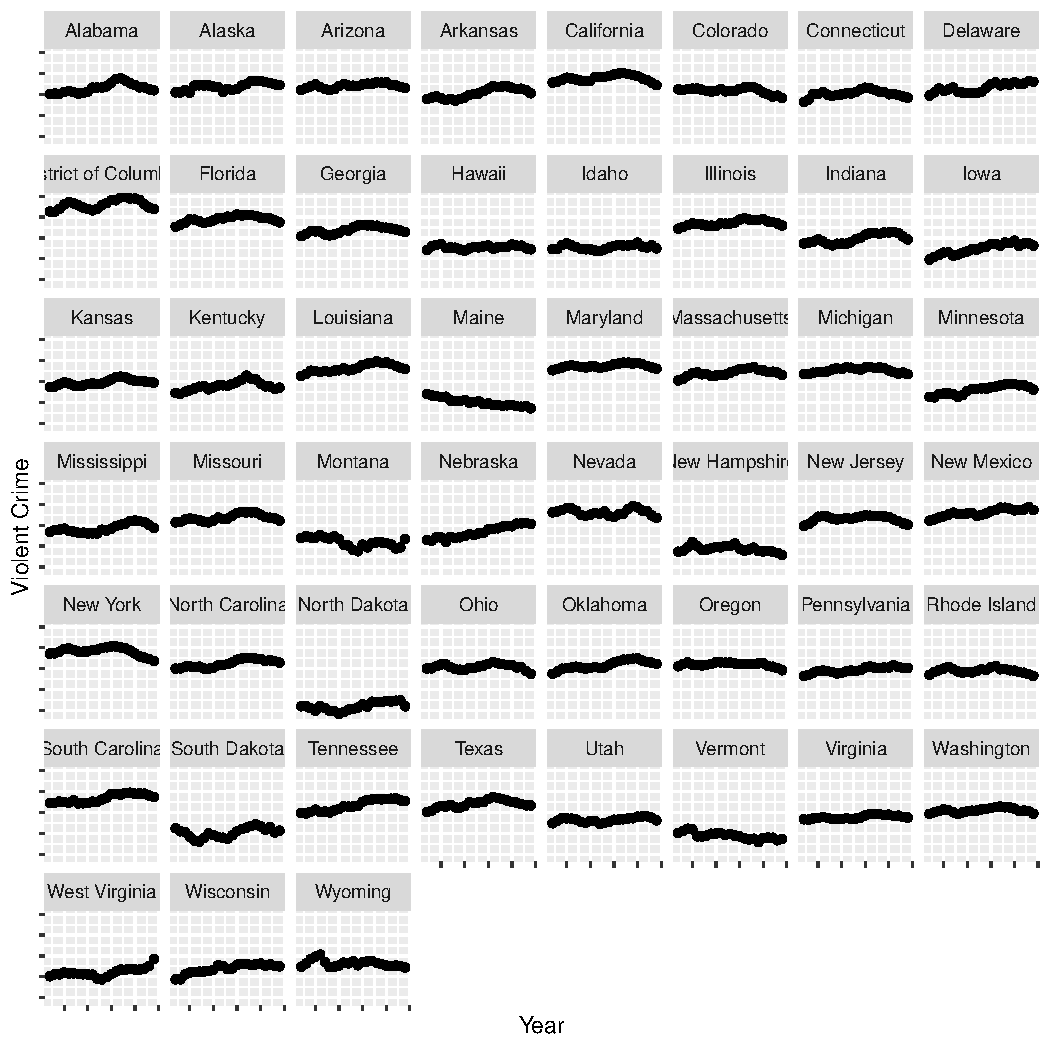
\includegraphics[width = 8cm]{plot/State_wrap}
\end{figure}
\end{frame}

\begin{frame}\frametitle{First regressions}
\begin{table}
\tiny
\begin{center}
\begin{tabular}{l c c c c }
\hline
  & \multicolumn{2}{c}{Violent Crime} & \multicolumn{2}{c}{Robbery}\\
 & Model 1 & Model 2 & Model 1 & Model 2 \\
\hline
(Intercept) & $6.13^{***}$  & $2.98^{***}$  & $4.87^{***}$  & $0.90$        \\
            & $(0.02)$      & $(0.54)$      & $(0.03)$      & $(0.77)$      \\
lawyes      & $-0.44^{***}$ & $-0.37^{***}$ & $-0.77^{***}$ & $-0.53^{***}$ \\
            & $(0.04)$      & $(0.03)$      & $(0.06)$      & $(0.05)$      \\
prisoners   &               & $0.00^{***}$  &               & $0.00^{***}$  \\
            &               & $(0.00)$      &               & $(0.00)$      \\
density     &               & $0.03^{*}$    &               & $0.09^{***}$  \\
            &               & $(0.01)$      &               & $(0.02)$      \\
income      &               & $0.00$        &               & $0.00^{***}$  \\
            &               & $(0.00)$      &               & $(0.00)$      \\
population  &               & $0.04^{***}$  &               & $0.08^{***}$  \\
            &               & $(0.00)$      &               & $(0.00)$      \\
afam        &               & $0.08^{***}$  &               & $0.10^{***}$  \\
            &               & $(0.02)$      &               & $(0.02)$      \\
cauc        &               & $0.03^{***}$  &               & $0.03^{*}$    \\
            &               & $(0.01)$      &               & $(0.01)$      \\
male        &               & $0.01$        &               & $0.03$        \\
            &               & $(0.01)$      &               & $(0.02)$      \\
\hline
R$^2$       & 0.09          & 0.56          & 0.12          & 0.60          \\
Adj. R$^2$  & 0.09          & 0.56          & 0.12          & 0.59          \\
Num. obs.   & 1173          & 1173          & 1173          & 1173          \\
RMSE        & 0.62          & 0.43          & 0.90          & 0.61          \\
\hline
\multicolumn{5}{l}{\scriptsize{$^{***}p<0.001$, $^{**}p<0.01$, $^*p<0.05$}}
\end{tabular}
\caption{Statistical models}
\label{table:coefficients}
\end{center}
\end{table}
\end{frame}

\begin{frame}\frametitle{Exploiting the Panel Structure}
\begin{table}
\tiny
\begin{center}
\begin{tabular}{l c c c }
\hline
 & Model 1 & Model 2 & Model 3 \\
\hline
(Intercept)               & $4.04^{***}$  & $3.09^{***}$  & $3.97^{***}$  \\
                          & $(0.39)$      & $(0.58)$      & $(0.47)$      \\
lawyes                    & $-0.05^{*}$   & $-0.29^{***}$ & $-0.03$       \\
                          & $(0.02)$      & $(0.03)$      & $(0.02)$      \\
prisoners                 & $-0.00$       & $0.00^{***}$  & $0.00$        \\
                          & $(0.00)$      & $(0.00)$      & $(0.00)$      \\
density                   & $-0.17^{*}$   & $-0.01$       & $-0.09$       \\
                          & $(0.09)$      & $(0.01)$      & $(0.08)$      \\
income                    & $-0.00$       & $0.00$        & $0.00$        \\
                          & $(0.00)$      & $(0.00)$      & $(0.00)$      \\
population                & $0.01$        & $0.04^{***}$  & $-0.00$       \\
                          & $(0.01)$      & $(0.00)$      & $(0.01)$      \\
afam                      & $0.10^{***}$  & $0.10^{***}$  & $0.03$        \\
                          & $(0.02)$      & $(0.02)$      & $(0.02)$      \\
cauc                      & $0.04^{***}$  & $0.04^{***}$  & $0.01$        \\
                          & $(0.01)$      & $(0.01)$      & $(0.01)$      \\
male                      & $-0.05^{***}$ & $-0.04^{*}$   & $0.07^{***}$  \\
                          & $(0.01)$      & $(0.02)$      & $(0.02)$      \\
State FE & YES & NO & YES \\
TIME FE & NO & YES & YES \\
\hline
R$^2$                     & 0.94          & 0.59          & 0.96          \\
Adj. R$^2$                & 0.94          & 0.58          & 0.95          \\
Num. obs.                 & 1173          & 1173          & 1173          \\
RMSE                      & 0.16          & 0.42          & 0.14          \\
\hline
\multicolumn{4}{l}{\scriptsize{$^{***}p<0.001$, $^{**}p<0.01$, $^*p<0.05$}}
\end{tabular}
\caption{Statistical models}
\label{table:coefficients}
\end{center}
\end{table}
\end{frame}


\begin{frame}\frametitle{Data: EmplUK}
Employment and Wages in the United Kingdom
\begin{itemize}
\item An unbalanced panel of 140 observations from 1976 to 1984
\item firm: firm index
\item year: year
\item sector: the sector of activity
\item emp: employment
\item wage: wages
\item capital: capital
\item output: output
\end{itemize}
\end{frame}

\begin{frame}\frametitle{Unbalanced Panel: Definitions}
\begin{itemize}
\item Unbalanced panel: Definition
\item What to do: Missing at random?
\end{itemize}
\end{frame}

\begin{frame}\frametitle{Unbalanced Panel: Solutions}
\begin{itemize}
\item Testing for missingness at random.
\item Missing at random
\begin{itemize}
\item Imputation
\item Full sample 
\item Non missing sample
\end{itemize}
\item Not missing at random
\begin{itemize}
\item Understand why?
\item Find an instrument
\end{itemize}
\end{itemize}
\end{frame}


\begin{frame}\frametitle{Description}
\begin{table}[!htbp] \centering 
\footnotesize
  \caption{} 
  \label{} 
\begin{tabular}{lccccccc} 
\\[-1.8ex]\hline 
\hline \\[-1.8ex] 
Statistic & \multicolumn{1}{c}{N} & \multicolumn{1}{c}{Mean} & \multicolumn{1}{c}{St. Dev.} & \multicolumn{1}{c}{Min} & \multicolumn{1}{c}{Pctl(25)} & \multicolumn{1}{c}{Pctl(75)} & \multicolumn{1}{c}{Max} \\ 
\hline \\[-1.8ex] 
firm & 1,031 & 73.204 & 41.233 & 1 & 37 & 110 & 140 \\ 
year & 1,031 & 1,979.651 & 2.216 & 1,976 & 1,978 & 1,981 & 1,984 \\ 
sector & 1,031 & 5.123 & 2.678 & 1 & 3 & 8 & 9 \\ 
emp & 1,031 & 7.892 & 15.935 & 0.104 & 1.180 & 7.020 & 108.562 \\ 
wage & 1,031 & 23.919 & 5.648 & 8.017 & 20.636 & 27.494 & 45.232 \\ 
capital & 1,031 & 2.507 & 6.249 & 0.012 & 0.221 & 1.501 & 47.108 \\ 
output & 1,031 & 103.801 & 9.938 & 86.900 & 97.098 & 110.603 & 128.365 \\ 
\hline \\[-1.8ex] 
\end{tabular} 
\end{table} 
\end{frame}

\begin{frame}\frametitle{Linear VS Log Specifications}
\begin{table}
\footnotesize
\begin{center}
\begin{tabular}{l c c }
\hline
 & Log & Linear \\
\hline
(Intercept)  & $0.34$        & $8.25^{**}$   \\
             & $(0.86)$      & $(3.11)$      \\
log(wage)    & $-0.37^{***}$ &               \\
             & $(0.06)$      &               \\
log(capital) & $0.81^{***}$  &               \\
             & $(0.01)$      &               \\
log(output)  & $0.48^{**}$   &               \\
             & $(0.18)$      &               \\
wage         &               & $-0.32^{***}$ \\
             &               & $(0.05)$      \\
capital      &               & $2.11^{***}$  \\
             &               & $(0.04)$      \\
output       &               & $0.02$        \\
             &               & $(0.03)$      \\
\hline
R$^2$        & 0.84          & 0.69          \\
Adj. R$^2$   & 0.84          & 0.69          \\
Num. obs.    & 1031          & 1031          \\
\hline
\multicolumn{3}{l}{\scriptsize{$^{***}p<0.001$, $^{**}p<0.01$, $^*p<0.05$}}
\end{tabular}
\caption{Statistical models}
\label{table:coefficients}
\end{center}
\end{table}
\end{frame}

\begin{frame}\frametitle{Fixed VS Random Effects}
\begin{table}
\footnotesize
\begin{center}
\begin{tabular}{l c c }
\hline
 & Fixed Effects & Random Effect \\
\hline
(Intercept)  & $2.20^{**}$   &       \\
             &  $(0.15)$     &       \\
log(wage)    & $-0.24^{***}$ &  $-0.61^{***}$             \\
             & $(0.05)$      &   $(0.03)$            \\
log(capital) & $0.61^{***}$  &  $0.56^{***}$            \\
             & $(0.07)$      &  $(0.02)$             \\
\hline
R$^2$        & 0.78          & 0.99          \\
Num. obs.    & 1031          & 1031          \\
\hline
\multicolumn{3}{l}{\scriptsize{$^{***}p<0.001$, $^{**}p<0.01$, $^*p<0.05$}}
\end{tabular}
\caption{Statistical models}
\label{table:coefficients}
\end{center}
\end{table}
\end{frame}

\begin{frame}\frametitle{Specification Problem}
\begin{itemize}
\item Choosing between random and fixed effects;
\item Durbin - Wu - Hausman Test 
\begin{equation}
H = (\beta_{FE} - \beta_{RE})' (Var(\beta_{FE}) - Var(\beta_{RE}))' (\beta_{FE} - \beta_{RE}) 
\end{equation}
\item $H \sim \chi_2(rank(Var(\beta_{FE}) - Var(\beta_{RE}))$
\end{itemize}
\end{frame}

\begin{frame}\frametitle{Data: US STATES PRODUCTION}
\begin{itemize}
\item state: state
\item year: year
\item region: the region
\item pcap: public capital stock
\item hwy: highway and streets
\item water: water and sewer facilities
\item util: other public buildings and structures
\item pc:private capital stock
\item gsp: gross state product
\item emp: labor input measured by the employment in nonagricultural payrolls
\item unemp: state unemployment rate
\end{itemize}
\end{frame}

\begin{frame}\frametitle{Specifications}
\begin{table}
\begin{center}
\begin{tabular}{l c c c }
\hline
 & Within & Between & First Difference \\
\hline
log(pcap)   & $-0.03$       & $0.18^{*}$   & $-0.01$       \\
            & $(0.03)$      & $(0.07)$     & $(0.05)$      \\
log(pc)     & $0.29^{***}$  & $0.30^{***}$ & $-0.03$       \\
            & $(0.03)$      & $(0.04)$     & $(0.02)$      \\
log(emp)    & $0.77^{***}$  & $0.58^{***}$ & $0.83^{***}$  \\
            & $(0.03)$      & $(0.06)$     & $(0.04)$      \\
unemp       & $-0.01^{***}$ & $-0.00$      & $-0.01^{***}$ \\
            & $(0.00)$      & $(0.01)$     & $(0.00)$      \\
(Intercept) &               & $1.59^{***}$ & $0.01^{***}$  \\
            &               & $(0.23)$     & $(0.00)$      \\
\hline
R$^2$       & 0.94          & 0.99         & 0.69          \\
Adj. R$^2$  & 0.94          & 0.99         & 0.69          \\
Num. obs.   & 816           & 48           & 768           \\
\hline
\multicolumn{4}{l}{\scriptsize{$^{***}p<0.001$, $^{**}p<0.01$, $^*p<0.05$}}
\end{tabular}
\caption{Statistical models}
\label{table:coefficients}
\end{center}
\end{table}
\end{frame}

\section{Nonlinear Panel}

\begin{frame}\frametitle{}
\end{frame}

\begin{frame}\frametitle{}
\end{frame}

\begin{frame}\frametitle{}
\end{frame}

\begin{frame}\frametitle{}
\end{frame}


\end{document}


